\documentclass[12pt,a4paper]{article}

% Pacotes essenciais
\usepackage[utf8]{inputenc}
\usepackage[T1]{fontenc}
\usepackage[portuguese]{babel}
\usepackage{geometry}
\usepackage{graphicx}
\usepackage{booktabs}
\usepackage{hyperref}
\usepackage{float}
\usepackage{titlesec}
\usepackage{amsmath}
\usepackage{subcaption}

% Configuração de margens
\geometry{top=2.5cm, bottom=2.5cm, left=3cm, right=3cm}

% Informações do Documento
\title{\textbf{Relatório Técnico de Ciência de Dados}\\ \large Integração Socioambiental, Identificação de Perfis e Validação Preditiva Atemporal para Esquistossomose no Brasil}
\author{
    Luiz Gabriel Correia dos Santos (15639682) \\
    Ana Paula de Abreu Batista (12688424) \\
    Italo Carlos Martins Bresciani (15461782)
}
\date{8 de junho de 2026}

\begin{document}

\maketitle

\begin{abstract}
Este relatório consolida a evolução da modelagem de dados aplicada à esquistossomose no Brasil. Atendendo às limitações identificadas em fases anteriores (focadas em desfechos clínicos), esta etapa integrou dados epidemiológicos (SINAN), ambientais (MapBiomas) e de saneamento (SNIS). O objetivo transitou da predição individual para a identificação de perfis de risco municipal. Utilizou-se o algoritmo \textit{K-Means} para mapear a assinatura de risco das cidades e \textit{Random Forest} com \textit{Undersampling} para prever a vulnerabilidade com base estritamente na infraestrutura e geografia. Análises de validação \textit{Out-of-Time} (2015-2025) comprovaram a atemporalidade das regras matemáticas descobertas, além de documentar a transição epidemiológica e a retração histórica da doença no território nacional.
\end{abstract}

\section{Introdução}
Historicamente, a esquistossomose mantém raízes profundas nas desigualdades de infraestrutura do Brasil. Relatórios anteriores deste projeto focaram na Análise Exploratória (EDA) do SINAN e na tentativa de predição de desfechos clínicos (Cura, Óbito). Tais etapas revelaram forte concentração geográfica da doença (especialmente em MG e ES) e apontaram o saneamento precário e as coleções hídricas como fatores latentes. 

Para superar as limitações dos dados puramente clínicos e o desbalanceamento das classes de desfecho, a abordagem metodológica foi reestruturada. A nova pergunta norteadora passou a ser: \textbf{quais características estruturais e ambientais fazem uma cidade se tornar um polo de transmissão da esquistossomose, e é possível prever esse risco?}

Para responder a essa questão, superamos a análise univariada e integramos dados do Ministério da Saúde, IBGE, MapBiomas e SNIS, modelando a dinâmica complexa entre população, água parada e saneamento.

\section{Base de Dados e Engenharia de Atributos}
Para capturar o padrão dinâmico da saúde pública, o escopo de dados foi ampliado e as seguintes bases foram concatenadas utilizando o período de referência inicial de \textbf{2011 a 2014} para treinamento:

\begin{itemize}
    \item \textbf{Saúde (SINAN via PySUS):} Notificações confirmadas por exame de fezes positivo (AN\_QUANT = 1).
    \item \textbf{População (IBGE):} Dados populacionais anuais, utilizados para nivelar a comparação entre municípios através do cálculo de \textit{Incidência por 100 mil habitantes}.
    \item \textbf{Geografia e Hidrografia (MapBiomas):} Foi aplicada uma engenharia de atributos crucial. Como grandes hidrelétricas e áreas de mineração não transmitem a doença (devido à profundidade e dinâmica da água), criou-se a métrica \texttt{açudes\_canais\_ha}. Esta variável isola a "água pequena" (açudes rurais e canais de irrigação), verdadeiro habitat do caramujo vetor.
    \item \textbf{Saneamento (SNIS):} Taxa de coleta de esgoto doméstico. Para lidar com valores faltantes, aplicou-se um \textit{pipeline} avançado de imputação: primeiro temporal (a cidade corrige seus anos faltantes baseada em seu histórico) e, em seguida, geoespacial (herança da mediana estadual/nacional do ano).
\end{itemize}

\section{Metodologia}

\subsection{Agrupamento de Perfis de Risco (Aprendizado Não Supervisionado)}
Para evitar distorções estatísticas, a base foi filtrada para conter apenas os municípios com ao menos um caso positivo no período. Utilizou-se o algoritmo \textbf{K-Means}, validado pelos métodos do Cotovelo e da Silhueta, determinando o número ideal de $K=5$ grupos (\textit{clusters}). O agrupamento avaliou simultaneamente incidência, população, área de açudes e taxa de esgoto, identificando automaticamente a assinatura do "Alto Risco".

\subsection{Modelagem Preditiva (Aprendizado Supervisionado)}
Após a clusterização, os rótulos gerados foram utilizados como alvo (\textit{target}) para um algoritmo \textbf{Random Forest}. O modelo foi "cego" em relação aos dados de saúde (incidência e casos) e treinado exclusivamente com variáveis ambientais e de infraestrutura. Devido ao forte desbalanceamento (poucas cidades de alto risco), aplicou-se a técnica de \textbf{Undersampling} na base de treino, forçando o modelo a aprender as diferenças estatísticas vitais sem adotar uma postura estática.

\subsection{Validação Temporal (Out-of-Time)}
Para testar o fenômeno do \textit{Concept Drift} (mudança de comportamento do mundo real no futuro), o modelo treinado nos dados de 2011-2014 foi desafiado a classificar o risco de municípios em duas janelas do "futuro": \textbf{2015-2019} e \textbf{2020-2025}.

\section{Resultados e Discussão}

\subsection{Os 5 Perfis da Esquistossomose no Brasil}
O \textit{K-Means} conseguiu isolar com clareza as dinâmicas demográficas e sanitárias do país:

\begin{enumerate}
    \item \textbf{Grandes Metrópoles (Cluster 3):} Populações milionárias (ex: SP e RJ), incidência nula. O algoritmo isolou os \textit{outliers} demográficos para não distorcer a análise.
    \item \textbf{Centros Médios com Grandes Represas (Cluster 4):} Confirma o paradoxo hídrico: maior área de água do país (hidrelétricas), porém incidência muito baixa (4,02/100k), provando que o caramujo não prolifera nessas condições.
    \item \textbf{Centros Urbanos Estruturados (Cluster 0):} Cidades de médio porte com boa cobertura de esgoto (76\%) e controle epidemiológico.
    \item \textbf{Cinturão de Vulnerabilidade (Cluster 1):} Menor cobertura de esgoto (31,5\%). Funciona como um risco latente; a incidência é moderada, mas o ambiente está propício a surtos.
    \item \textbf{Epicentro da Doença - Alto Risco Absoluto (Cluster 2):} Cidades muito pequenas, baixíssima água detectada pelo satélite macro (açudes periféricos) e taxa de esgoto de gabinete mediana (62,9\%). Onde a incidência explodiu para impressionantes \textbf{778,02 casos por 100 mil habitantes}.
\end{enumerate}

\begin{table}[H]
    \centering
    \caption{Perfil médio das variáveis estruturais e epidemiológicas para cada grupo (cluster) identificado.}
    \label{tab:perfil_clusters}
    \renewcommand{\arraystretch}{1.2} % Dá um leve respiro entre as linhas
    % O comando abaixo ajusta a tabela para a largura do texto (\textwidth)
    \resizebox{\textwidth}{!}{%
    \begin{tabular}{@{}lcccc@{}}
        \toprule
        \textbf{Perfil (Cluster)} & \textbf{Incidência} & \textbf{Açudes/Canais} & \textbf{Taxa de Esgoto} & \textbf{População} \\
        & \textbf{(por 100k hab.)} & \textbf{(Hectares)} & \textbf{Média (\%)} & \textbf{Média} \\
        \midrule
        0 - Centros Estruturados & 19,94 & 41,02 & 76,34 & 99.484 \\
        1 - Cinturão de Vulnerabilidade & 11,30 & 61,70 & 31,57 & 68.008 \\
        2 - Epicentro (Alto Risco) & 778,02 & 3,44 & 62,97 & 11.101 \\
        3 - Grandes Metrópoles & 0,36 & 150,67 & 68,39 & 9.005.051 \\
        4 - Centros com Represas & 4,02 & 1.219,80 & 47,95 & 146.357 \\
        \bottomrule
    \end{tabular}%
    } % Fecha o resizebox
\end{table}

\begin{figure}[H]
    \centering
    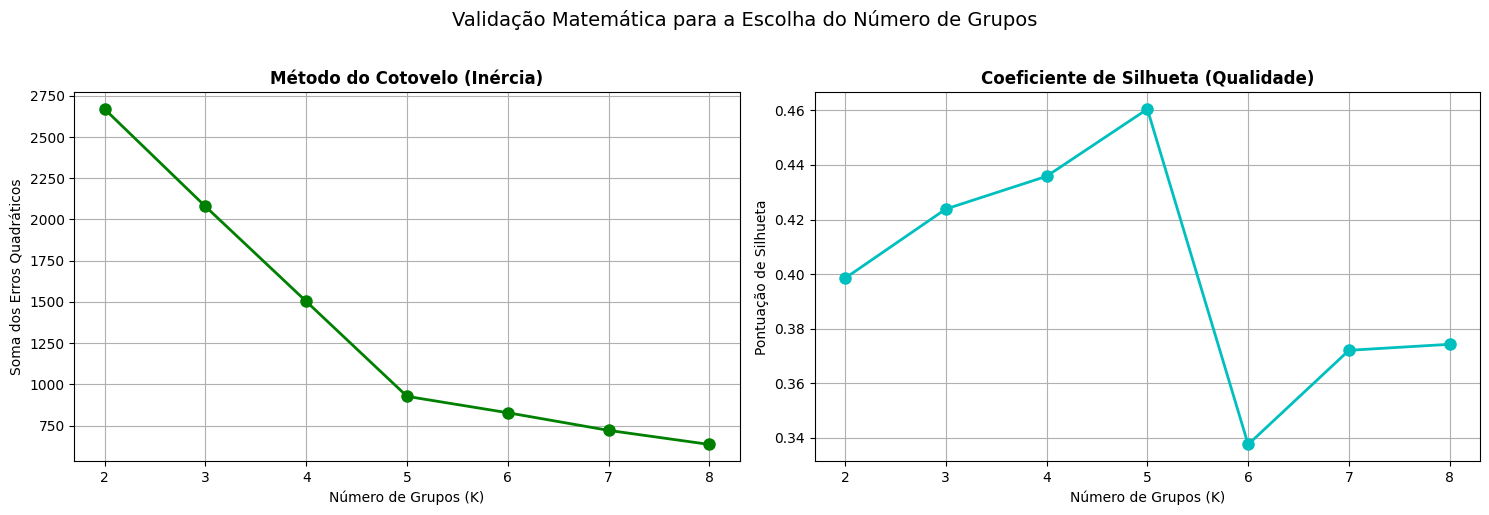
\includegraphics[width=0.9\textwidth]{cotovelo.png}
    \caption{Gráficos de Validação Matemática para a escolha do K cluters}
    \label{fig:cotovelo_clusters}
\end{figure}

\begin{figure}[H]
    \centering
    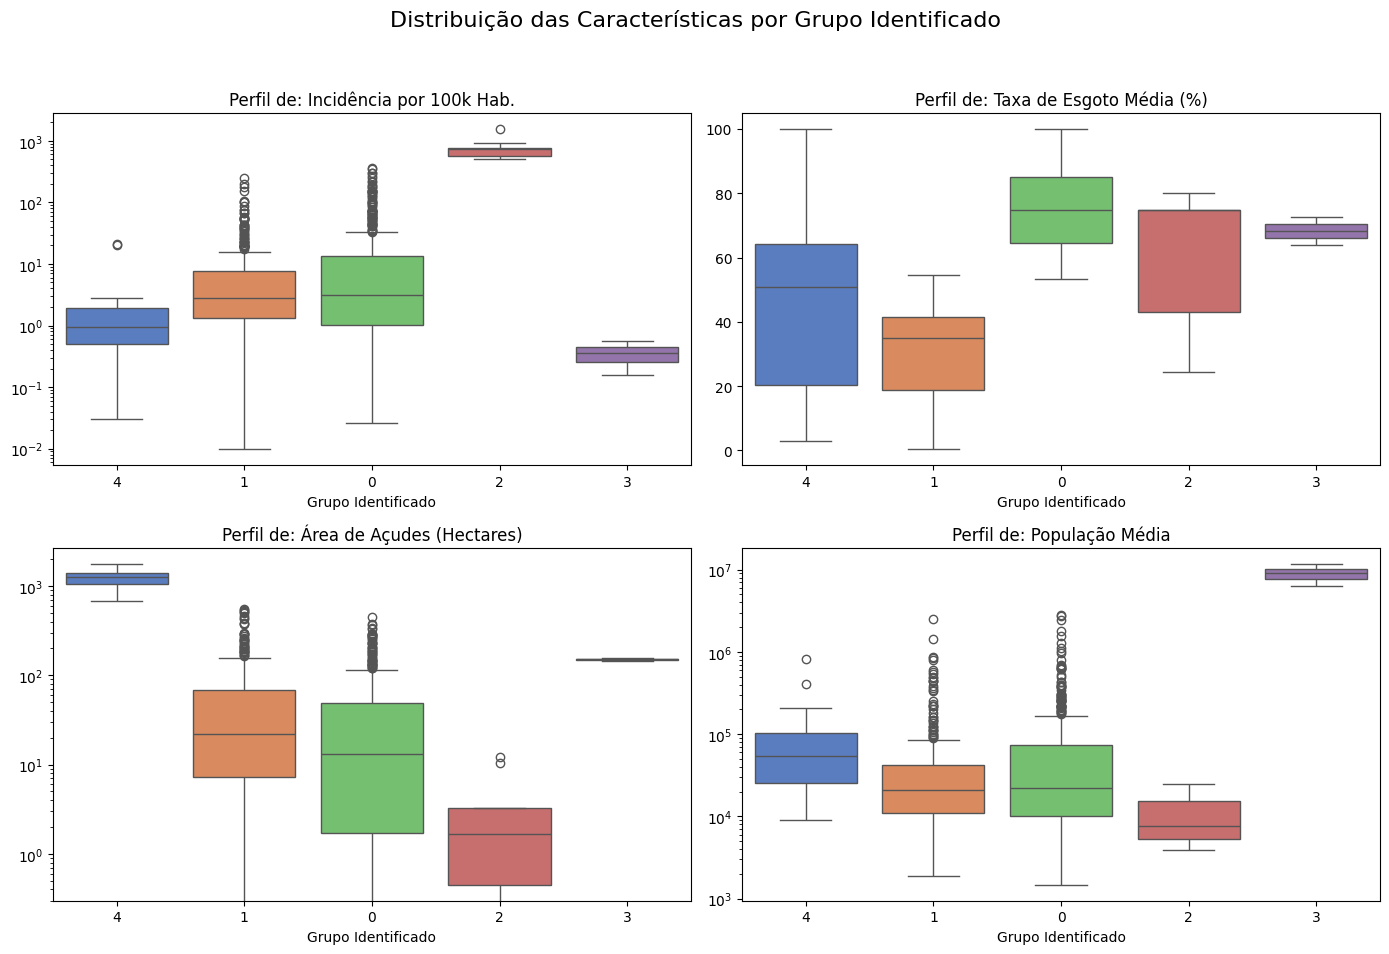
\includegraphics[width=0.9\textwidth]{boxplots.png}
    \caption{Gráficos de Boxplots das Características por cluster}
    \label{fig:cotovelo_clusters}
\end{figure}

\subsection{A Importância das Variáveis}
A floresta aleatória balanceada revelou que a variável \texttt{açudes\_canais\_ha} (27,30\% de importância) e \texttt{taxa\_esgoto\_media} (26,42\%) assumiram o protagonismo. A geografia natural (\texttt{natural\_ha}) ficou em terceiro (21,55\%). 

\begin{figure}[H]
    \centering
    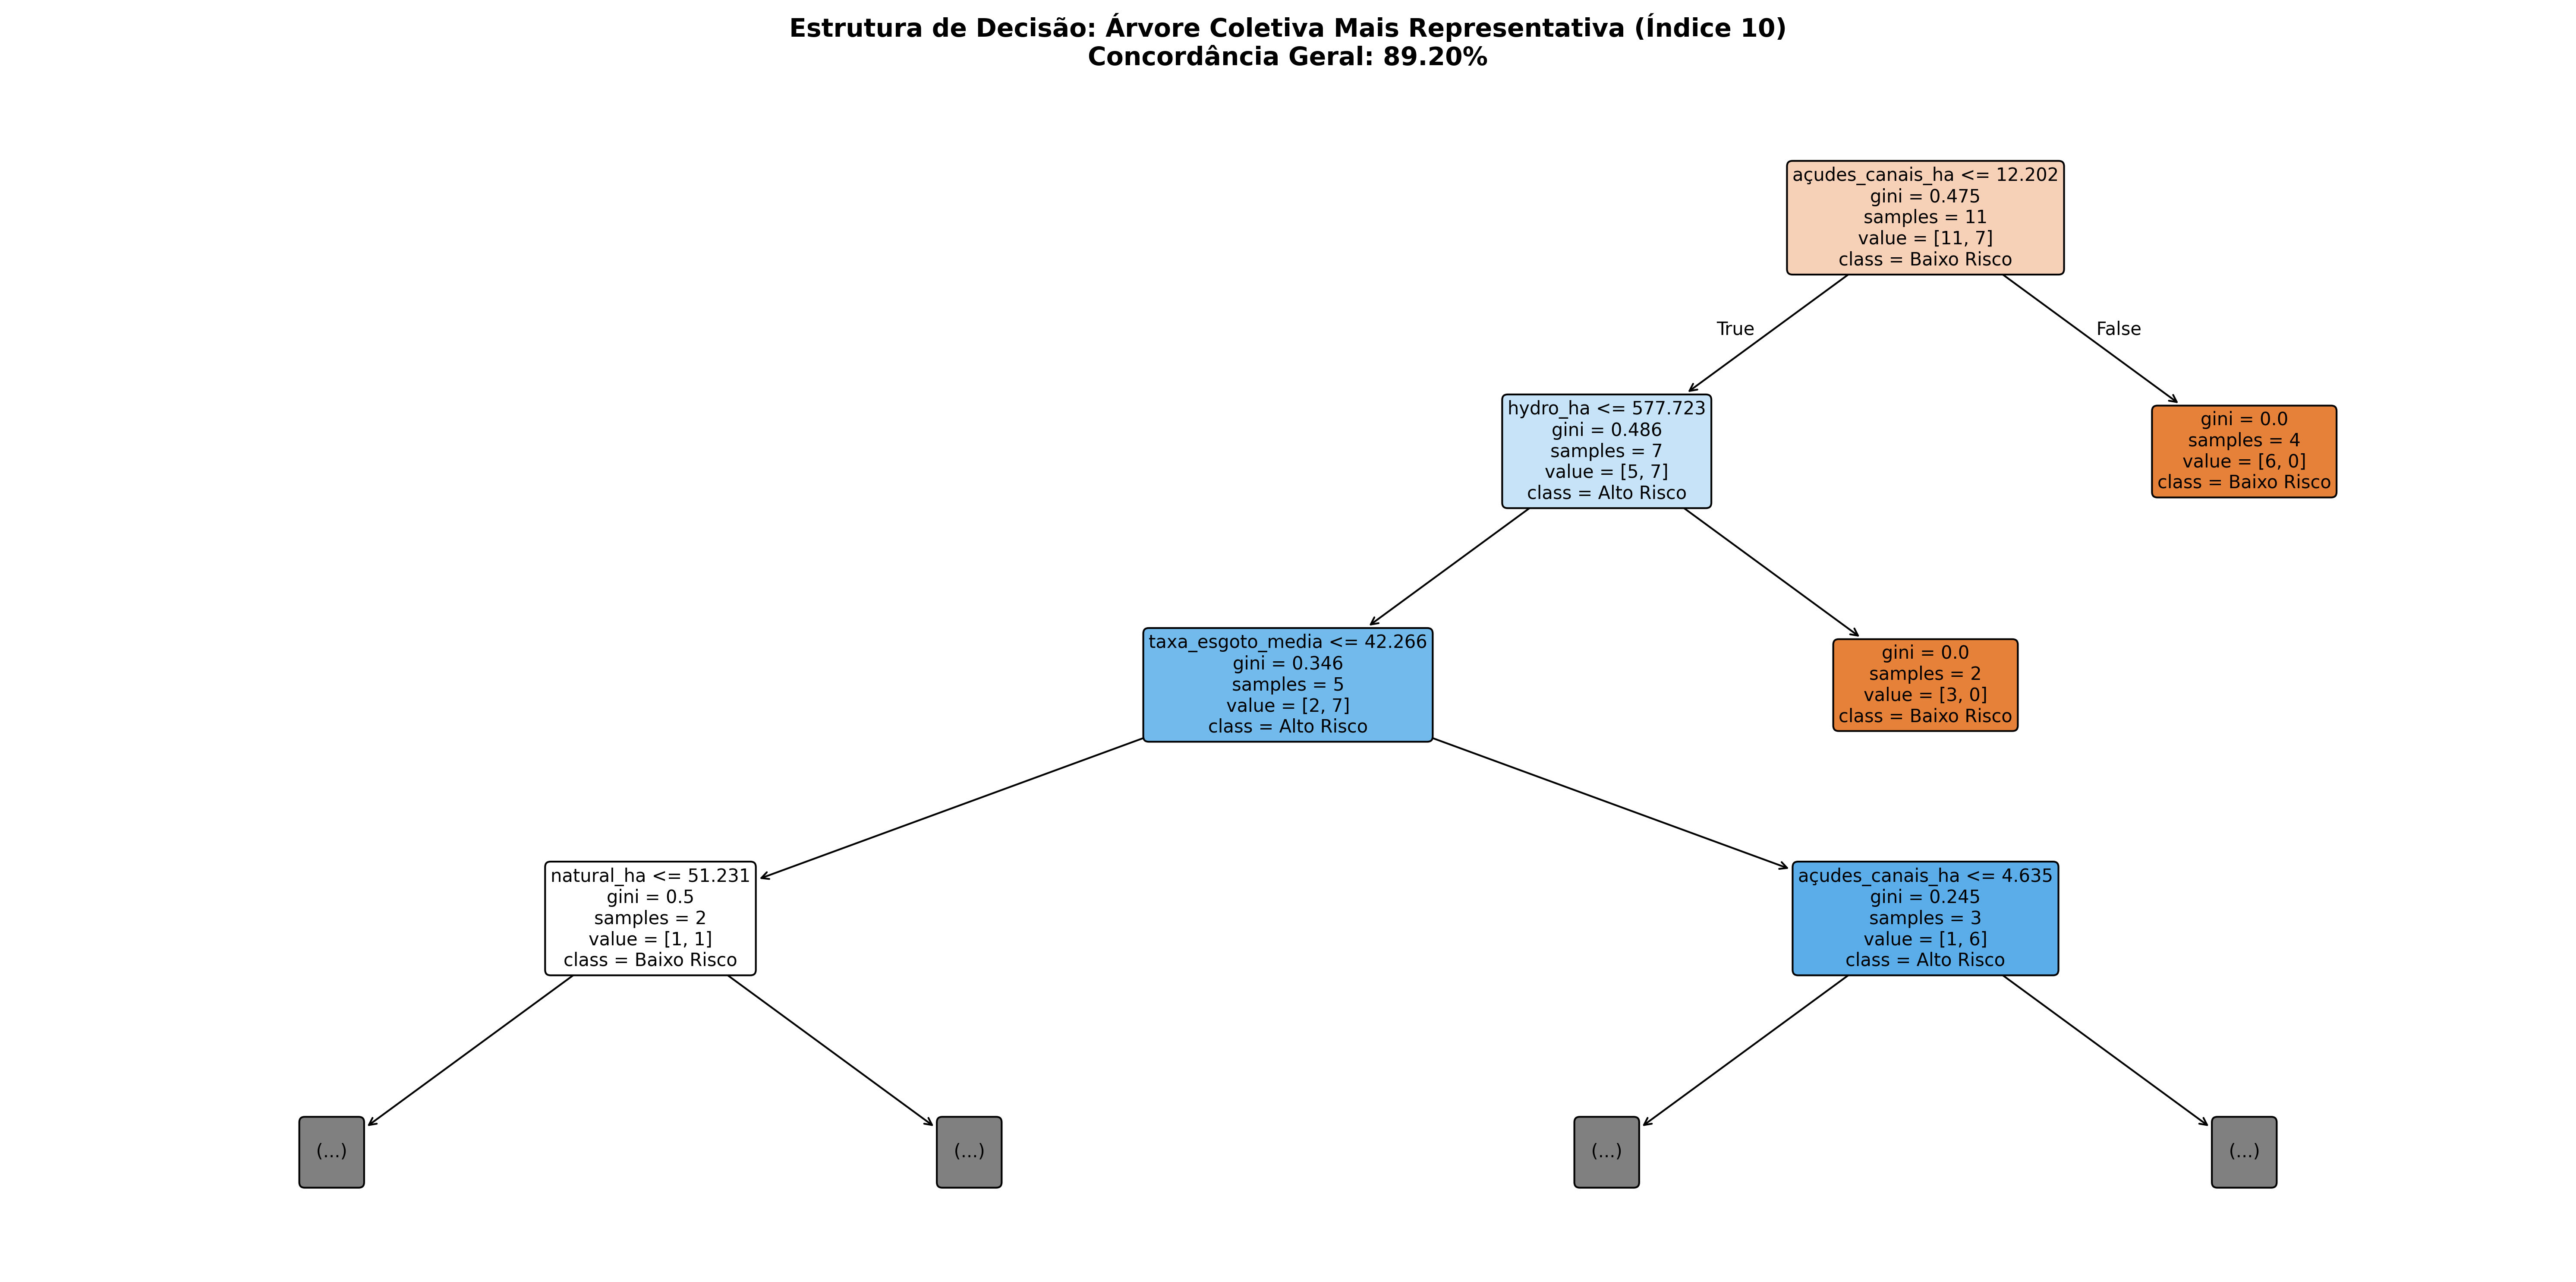
\includegraphics[width=0.9\textwidth]{arvore.png}
    \caption{Árvore mais representativa encontrada no Random Forest}
    \label{fig:cotovelo_clusters}
\end{figure}

A modelagem evidenciou uma limitação crítica nos indicadores oficiais de infraestrutura. Municípios endêmicos em Minas Gerais, a exemplo de Dom Silvério, registram 100\% de cobertura de esgotamento sanitário no SNIS. Em abordagens preditivas convencionais, esse índice gerava falsos negativos ao mascarar a vulnerabilidade real. A análise demonstrou, contudo, que a coleta de esgoto concentrada nos centros urbanos não interrompe o ciclo de transmissão quando as populações periféricas e rurais permanecem expostas a redes de pequenos açudes antrópicos.


\subsection{Validação Temporal e a Retração Histórica}
O ecossistema da doença foi encurralado na última década. No treino (2011-2014) havia 9 municípios no polo absoluto de risco; em 2015-2019 caiu para 6; e em 2020-2025 colapsou para apenas 1 município.

No teste \textit{Out-of-Time}, o modelo obteve:
\begin{itemize}
    \item \textbf{Acurácia Global Estável:} 82,26\% no teste original, 75,33\% no quinquênio seguinte e 73,96\% na década atual.
    \item \textbf{Recall Cirúrgico:} No horizonte 2020-2025, o modelo cravou o alerta na única cidade doente do Brasil (Dom Silvério), garantindo \textbf{100\% de Recall}.
\end{itemize}

\begin{figure}[H]
    \centering
    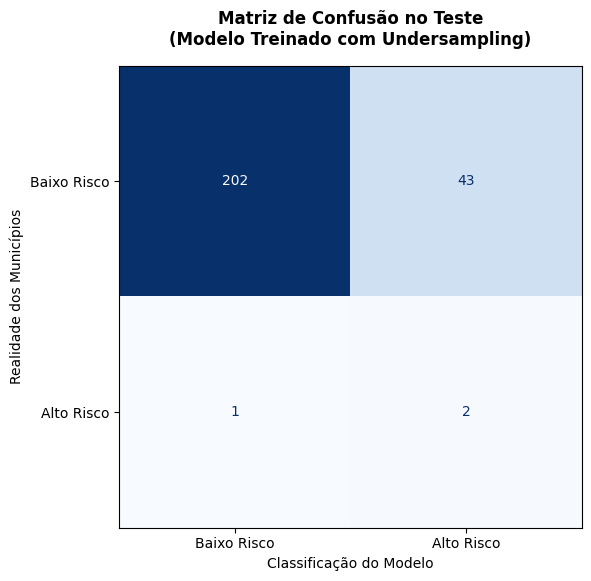
\includegraphics[width=0.5\textwidth]{matrizdeconfusao.png}
    \label{fig:matriz_orig}
\end{figure}

O modelo gerou dezenas de Falsos Positivos ao olhar para o futuro. Para a epidemiologia, isso atua como um \textbf{mapa de vigilância ativa} (Screening). O modelo alertou que essas cidades continuam com o ambiente perfeito para o parasita, e sua atual baixa incidência é mérito de intervenções de saúde, mantendo a vulnerabilidade estrutural latente.

\begin{figure}[H]
    % --- Matrizes do Futuro (lado a lado na base) ---
        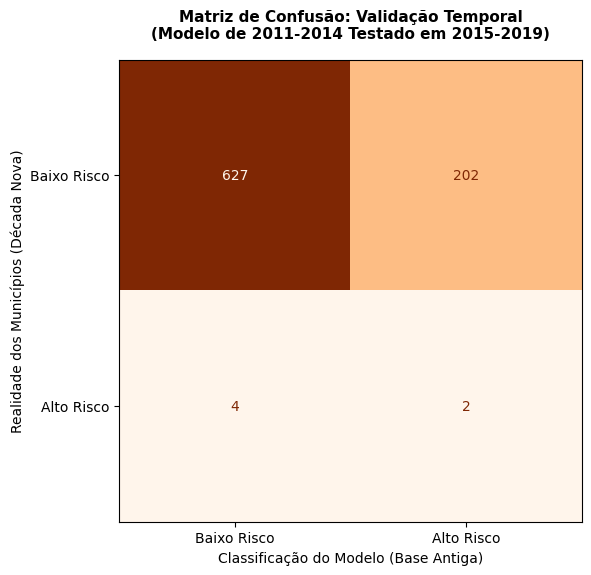
\includegraphics[width=0.5\textwidth]{2015-2019.png}
        \label{fig:matriz_1519}
    \hfill % Empurra as imagens para as bordas, dando um espaço no meio
        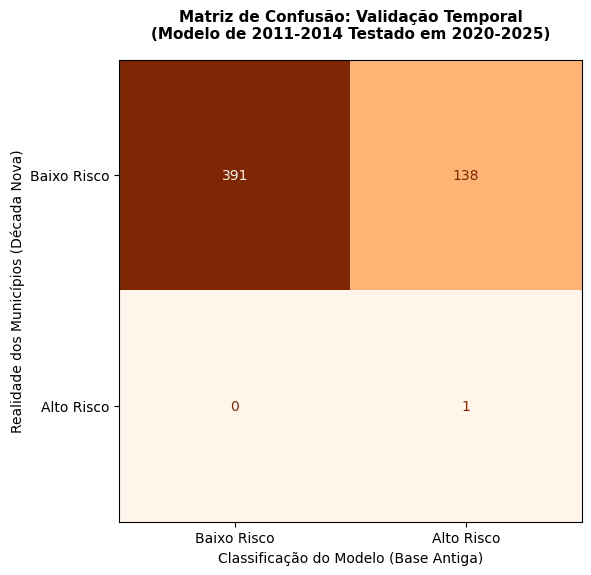
\includegraphics[width=0.5\textwidth]{2020-2025.png}
        \label{fig:matriz_2025}
    
    % Legenda geral da figura inteira
    \caption{Desempenho do modelo na validação temporal (Out-of-Time). Na figura em azul, o desempenho no teste cego original. Nas duas figuras em laranja, a aplicação no futuro evidencia a captura cirúrgica do alvo crítico (100\% de Recall na década atual) e o extenso mapeamento preventivo de vulnerabilidade latente (falsos positivos).}
    \label{fig:matriz_temporal}
\end{figure}

\section{Conclusão e Recomendações}
O projeto atingiu o ápice do rigor científico ao transpor a barreira dos dados univariados. Comprovou-se matematicamente que a infraestrutura (açudes e esgotamento) possui alto sinal preditivo para a esquistossomose, superando as limitações apontadas nos relatórios iniciais da disciplina.

A estrutura lógica do modelo é \textbf{atemporal}, pois a assinatura socioambiental de contágio não mudou nas últimas décadas. Contudo, devido ao \textit{concept drift} ocasionado pela retração histórica e avanço da medicina básica, a modelagem atual tornou-se um radar muito sensível. A recomendação prática é o \textbf{retreino do algoritmo com a base pós-2020}, permitindo recalibrar os pontos de corte da árvore de decisão para distinguir a vulnerabilidade latente (risco ambiental) das áreas de surto ativo (risco crônico).

\end{document}